\setchapterpreamble[u]{\margintoc}
\chapter{Երկրաչափական մեկնաբանություն}
\labch{geometry}

\emergencystretch 2em

\section{Գծային ձևափոխու\-թյուն\-ները երկրաչափորեն}

Նախորդ թեմայից հետո ծագում է հետևյալ հարցը․

\textit{— Ուրեմն մատրից $=$ թվերի աղյուսակ, այդքան բա՞ն}

Շտապենք հանգստացնել․ պատասխանն է՝ ոչ, բացարձակապես ոչ, մատրիցներն ընդամենը թվերի աղյուսակներ չեն, և Դուք ստիպված չեք լինելու ձանձրալի ու անհետաքրքիր թվեր բազմապատկելով զբաղվել։ 
Ինչպես ամեն վեկտոր ոչ այլ ինչ է, քան տարածության մեջ ինչ-որ մի սլաք, այդպես էլ մատրիցները՝ գծային ձևափոխությունները, գեղեցիկ երկրաչափական գաղափարներ են։ 

Պատկերացրեք՝ թղթի վրա նկարել ենք կոորդինատային առանցքները և մի քանի վեկտորներ։ Եթե ենթադրենք, որ թուղթը ռեզինից է, և ձգել-սեղմելուց չի պատռվում, այլ լոճվում է, ապա կարող ենք այն, օրինակ,
\begin{itemize}
    \item պտտել $40^\circ$-ով
    \item ձախ ու աջ կողմերից ձեռքով բռնել և ձգել
    \item վերևից ու ներքևից բռնել և ներս սեղմել
    \item վերևից ու ներքևից բռնել և ներս սեղմել, ապա $15^\circ$-ով պտտել
\end{itemize}
\begin{marginfigure}    \begin{center}

\includegraphics[width=0.55\textwidth, height=\textheight, keepaspectratio]{chapters/chapter 3/khinkali.png}
\end{center}
\caption*{ի՞նչ կլինի խինկալիների հետ, եթե գուլ\-պան ձախից ու աջից բռնենք և քաշենք}
\end{marginfigure}
Ամեն անգամ թղթի վրայի բոլոր վեկտորները իրենց նախորդ դիրքի համեմատ կպտտվեն, կձգվեն, կսեղմվեն, այսինքն՝ կձևափոխվեն ինչպես մնացած վեկտորները։  Ահա հենց այդպիսի ազդեցություն է լինում, երբ տարածության մեջ ինչ-որ վեկտորներ բազմապատկում ենք մատրիցով։

\begin{figure}[h]
    \centering
    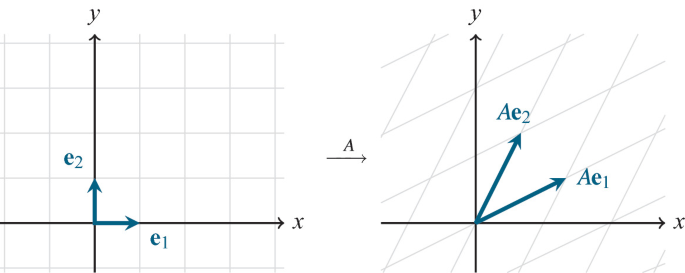
\includegraphics[width=0.75\linewidth]{chapters/chapter 3/viz ex.png}
\end{figure}

Իրոք, ի՞նչ է տեղի ունենում, երբ օրինակ՝ $2\times 2$ չափանի $A$ մատրիցը կիրառում ենք $\vv\in\R^2$ վեկտորի վրա․ ստանում ենք մեկ այլ՝ նոր $\vu=A\vv\in\R^2$ վեկտոր։ Այս նոր, ձևափոխված $\vu$ վեկտորը նույն հին ու բարի $\vv$-ն է՝ պարզապես ինչ-որ անկյան տակ \textbf{պտտած, ձգած} կամ \textbf{սեղմած} և, հնարավոր է, \textbf{շրջած} ({\rm flip} արած)։ Թե քանի աստիճանով պտտած և հորիզոնական/ուղղաձիգ ուղղությամբ քանի անգամ է այն ձգած՝ կախված է մատրիցի մեջ գրված թվերից, բայց բուն գաղափարն այն է, որ տրված $A$ մատրիցը \textit{ինչ գործողություններ որ անում է որևէ վեկտորի հետ, նույն \marginnote{գործողություն $=$ պտույտ, ձգում, սեղ- \linebreak մում, շրջում (որոշ հերթականությամբ)}գործողությունները անում է նաև բոլոր մյուս վեկտորների հետ,} այն այդ վեկտորների վրա կիրառելիս։

Այլ կերպ ասած՝ եթե վեկտորները տարածության մեջ սլաքներ են, ապա մատրիցները այդ սլաքների պտտումները, ձգումները, սեղմումներն ու շրջումներն են։

\begin{figure}[t]
    \label{mona}
    \centering
    % \subfloat[\centering label 1]{{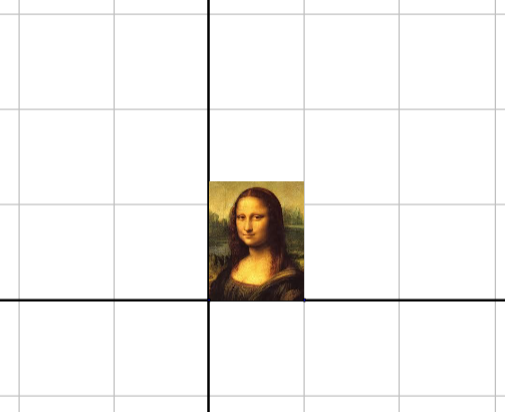
\includegraphics[width=0.4\linewidth]{chapters/chapter 3/mona_1.png} }}%
    \subfloat{{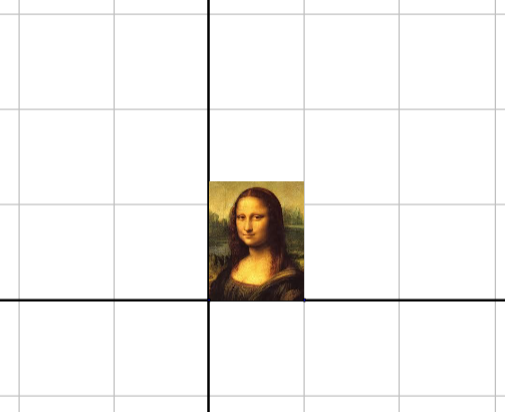
\includegraphics[width=0.4\linewidth]{chapters/chapter 3/mona_1.png} }}%
    \qquad
    \subfloat{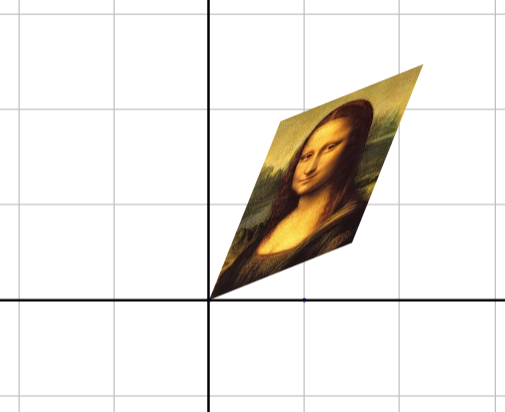
\includegraphics[width=0.4\linewidth]{chapters/chapter 3/mona_2.png}} %
    \caption*{Մոնա Լիզան՝ $$M = \begin{bmatrix}
        1.5 & 0.6 \\ 0.6 & 1.5
    \end{bmatrix}$$ մատրիցից առաջ և հետո \href{https://www.geogebra.org/m/pDU4peV5}{(փորձել)}}
\end{figure}

Հաջորդ թեմայում կպարզենք նաև, թե ինչպես մատրիցի թվերին նայելով հասկանալ, թե այն ինչպե՞ս է ձևափոխում տարածությունը։ Մինչ այդ օգտակար կլինի փորձարկել տարբեր մատրիցներ և սեփական աչքով տեսնել դրանց կատարած ձևափոխությունները՝ անցնելով \href{visualize-it.github.io/linear_transformations/simulation.html}{այստեղ} կամ \href{https://shad.io/MatVis}{այստեղ}։

\question{Ի՞նչ են անում հետևյալ գծային ձևափոխությունները․}
\[
\begin{bmatrix}
1& 2 \\ 0 & 1
\end{bmatrix},
\qquad 
\begin{bmatrix}
3& 0 \\ 0 & 3
\end{bmatrix},
\qquad 
\begin{bmatrix}
3 & 1 \\ 0 & 1
\end{bmatrix},
\qquad \begin{bmatrix}
-1 & -1 \\ -1 & 1
\end{bmatrix}
\]

\warning{Երբ ասում ենք՝ մատրիցները պտտում, ձգում, սեղմում, շրջում են վեկտորները, նկատի չունենք, որ ամեն մատրից միայն սեղմում է կամ միայն շրջում․ մատրիցը կարող է, օրինակ՝
\begin{enumerate}
    \item նախ պտտել տարածությունը,
    \item հետո սեղմել հորիզոնական ուղղությամբ,
    \item հետո նորից պտտել,
    \item ապա ձգել ուղղաձիգ ուղղությամբ։
\end{enumerate}}



\section{Ձևափոխությունների արտադրյալ}

Փաստորեն՝ մատրիցը վեկտորով բազմապատկել նշանակում է որոշակի ձևով պտտել-ձգել վեկտորը։ Իսկ ի՞նչ է նշանակում մատրիցը բազմա\-պատ\-կել մատրիցով։


Ենթադրենք $\mathbf{v} \in \R^2$ որևէ վեկտոր է, իսկ $A \in \R^{2 \times 2}$, $B \in \R^{2 \times 2}$ ինչ-որ մատրիցներ են։ 

\begin{figure}
\centering
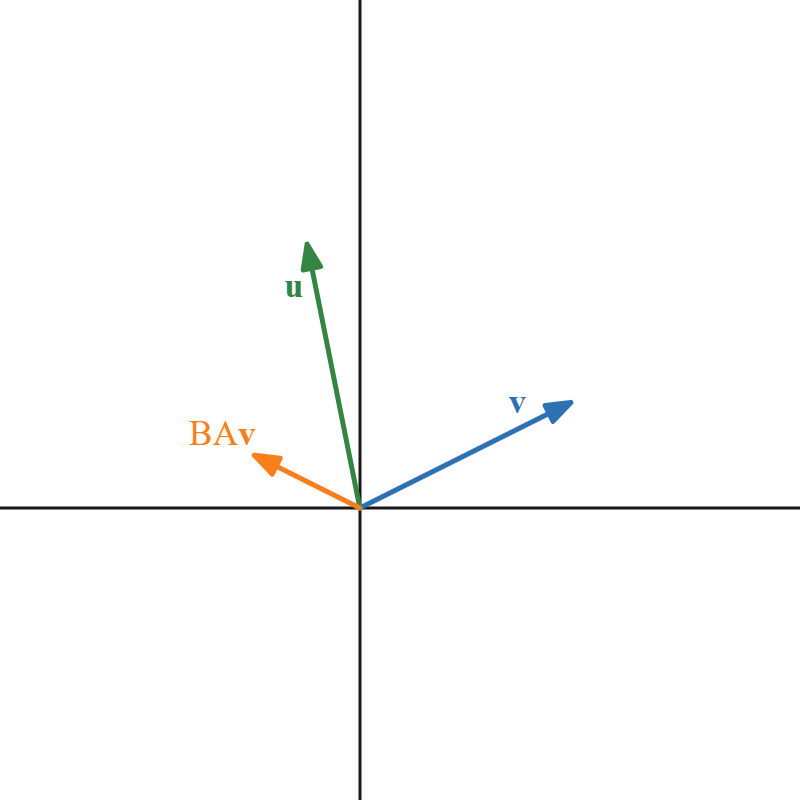
\includegraphics[width=0.5\linewidth]{chapters/chapter 3/viz matrix mult.png}
\end{figure}

Եթե $\vv$ վեկտորի վրա կիրառենք $A$-ն՝ $\vv$-ն կձևափոխվի, և կստանանք մի նոր վեկտոր՝ $A\vv$։ Հարմարության համար ստացվածը նշանակենք $\mathbf{u}$-ով: Եթե հիմա $\vu$-ի վրա կիրառենք $B$-ն, ապա այն կձևափոխի $\vu$-ն, և կունենանք մի նոր վեկտոր՝ $B\vu$: 

Արդյունքում ստացանք՝ 
\[
B\vu = B(A\vv) = (BA)\vv,
\]
ասել է թե՝ $BA$ մատրիցը կիրառած $\vv$ վեկտորի վրա։ Փաստորեն $B$ և $A$ գծային ձևափոխությունների (մատրիցների) արտադրյալը կիրառելը նույնն է, ինչ եթե նախ կիրառես $A$-ն, ապա $B$-ն․ 
\[
BA \; = \; \Big(\;\text{կիրառիր } A\text{-ն, ապա } B\text{-ն}\;\Big)
\]

\begin{marginfigure}    \begin{center}
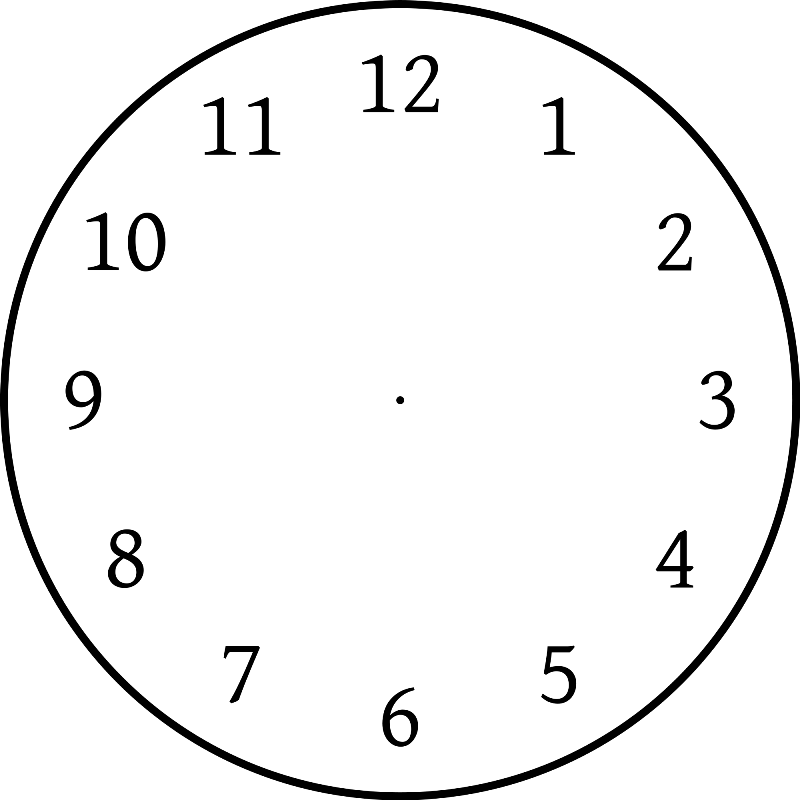
\includegraphics[width=0.55\textwidth, height=\textheight, keepaspectratio]{chapters/chapter 3/clock.png}
\end{center}
\caption*{պտույտներն ու շրջումները հարմար է պատկերացնել ժամացույցի վրա}
\end{marginfigure}

\question{Պատկերացրեք՝ $A$-ն $30^\circ$-ով պտույտն է, իսկ $B$-ն՝ ուղղաձիգի նկատմամբ հայելային արտապատկերումը (շրջումը)։ Ի՞նչ է ցույց տալիս $AB$-ն։ Իսկ $BA$՞-ն։}

Ենթադրենք $A$-ն այն մատրիցն է, որը վեկտորները պտտում է $30^\circ$-ով (ժամսլաքի ուղղությամբ),  $B$-ն՝ $50^\circ$-ով, իսկ $C$-ն՝ $260^\circ$-ով։

\question{Ի՞նչ է անում $BA$ մատրիցը։ Իսկ $CBA$՞-ն։}



\section{Միավոր մատրից}

Եթե օրինակ մատրիցը հորիզոնական ուղղությամբ $2$ անգամ ձգում է բոլոր վեկտորները՝
\[
\begin{bmatrix}
    x \\ y
\end{bmatrix}
\mapsto 
\begin{bmatrix}
    2x \\ y
\end{bmatrix}
\]
իսկ ուղղաձիգ ուղղությամբ ոչինչ չի անում, ապա  այն վեկտորները, որոնց առաջին կոորդինատը $0$ է,\marginnote{$x$-երի առանցքի վրայի վեկտորները} ձևափոխության արդյունքում չեն փոփոխվում։

Իսկ ո՞ր մատրիցն է, որ բոլոր վեկտորները թողնում է իրենց տեղերում, ոչ մեկին չի փոփոխում։ Փորձենք պարզել։

\begin{definition}
$A$-ն կոչվում է \textbf{քառակուսային} մատրից, եթե նրա տողերի ու սյուների թիվը համընկնում է։\marginnote{$n\times n$ չափանի}
\end{definition}

\begin{definition}
$A$ քառակուսային մատրիցը կոչվում է \textbf{սիմետրիկ} (համաչափ), եթե $A^T=A$:\marginnote{շրջելուց հետո մնում է նույնը}
\end{definition}

\begin{example} 
Հետևյալ մատրիցը սիմետրիկ է (ուստի և քառակուսային)՝
\[
A = \begin{bmatrix}
2 & 0 & 1 \\
0 & -3 & 4 \\
1 & 4 & 6 \\
\end{bmatrix}
\]
\end{example}

Եթե մտովի գիծ տանենք $A$ մատրիցի վերևի ձախ անկյունից դեպի ներքևի աջ անկյունը, կստանանք նրա \textit{գլխավոր անկյունագիծը,} որի նկատմամբ $A$-ն սիմետրիկ է․ $0$-ի համաչափը $0$-ն է, $1$-ի համաչափը՝ $1$-ը, և այլն։

\begin{definition}
$A$ մատրիցի \textbf{գլխավոր անկյունագիծ} (կամ պարզապես \textbf{անկյունագիծ}) ենք անվանում նրա $a_{ii}$ տեսքի տարրերը, որոնց տողերի ու սյուների համարները\marginnote{$A$-ն կարող է չլինել քառակուսային} համընկնում են՝  $a_{11}$, $a_{22}$, $\dots$:
\end{definition}

Մյուս անկյունագիծը՝ վերևի աջ անկյունից դեպի ներքևի ձախ, կոչվում է \textit{երկրորդ անկյունագիծ։}

\begin{example}
Այստեղ կարմիրով նշված է գլխավոր անկյունագիծը՝
\[
{\displaystyle {\begin{bmatrix}\color {red}{1}&0&0\\0&\color {red}{1}&0\\0&0&\color {red}{1}\end{bmatrix}}\qquad {\begin{bmatrix}\color {red}{1}&0&0&0\\0&\color {red}{1}&0&0\\0&0&\color {red}{1}&0\end{bmatrix}}\qquad {\begin{bmatrix}\color {red}{1}&0&0\\0&\color {red}{1}&0\\0&0&\color {red}{1}\\0&0&0\end{bmatrix}}\qquad {\begin{bmatrix}\color {red}{1}&0&0&0\\0&\color {red}{1}&0&0\\0&0&\color {red}{1}&0\\0&0&0&\color {red}{1}\end{bmatrix}}}
\]
իսկ այստեղ՝ երկրորդ անկյունագիծը․
\[
{\displaystyle {\begin{bmatrix}0&0&\color {red}{1}\\0&\color {red}{1}&0\\\color {red}{1}&0&0\end{bmatrix}}}
\]
\end{example}

Վերադառնանք մեր հարցին․ ո՞ր մատրիցով բազմապատկելիս է ամեն բան մնում իր տեղում։

\begin{definition}
$n$-չափանի \textbf{միավոր մատրից} է կոչվում այն քառակուսային մատրիցը\marginnote{կասենք՝ \textit{նույնական ձևափոխություն}}, որի անկյունագծի վրա $1$-եր են, իսկ մնացած բոլոր տեղերում՝ $0$-ներ։
\end{definition}

$n$-չափանի միավոր մատրիցը կարճ կնշանակենք $I_n$-ով։

\begin{example}
\[
I_3 = \begin{bmatrix}
1 & 0 &0  \\
0 & 1 &0\\
0 &0& 1\\
\end{bmatrix}
\]
\end{example}

Դժվար չէ ապացուցել, որ միավոր մատրիցով բազմապատկելիս վեկտորները չեն փոխվում՝
\[
I_n \vv = \vv \qquad \text{եթե }\vv\in\R^n
\]

Եվ ավելին, ցանկացած $A\in\R^{m\times n}$ մատրիցի և միավոր մատրիցի արտադրյալը ինքը՝ $A$-ն է․
\[ I_m A = A = A I_n \]

\question{Ի՞նչ են նշանակում $I_mA$ և $AI_n$ արտադրյալները։}



\section{Հակադարձ}

\question{Անին իր հասակը բազմապատկեց $4$-ով, հանեց $15$, բաժանեց $13$-ի և ստացավ $53$ սմ։ Որքա՞ն է Անիի հասակը։}

Պատասխանը գտնելու համար քայլերը կանենք հակառակ հերթակա\-նու\-թյամբ՝ $53$-ը կբազմապատկենք $13$-ով, կգումարենք $15$ և կբաժանենք $4$-ի, արդյունքում կստանանք Անիի հասակը։ 

Իսկ ի՞նչ, եթե ունենք մի $\vv\in \R^n$ անհայտ վեկտոր, որը ինչ-որ $A$ մատրիցով ենթարկվել է գծային ձևափոխության։ Ինչպե՞ս ունենալով $A\vv$-ն՝ վերականգնենք սկզբնական $\vv$ վեկտորը։

\begin{figure}[h]
\centering
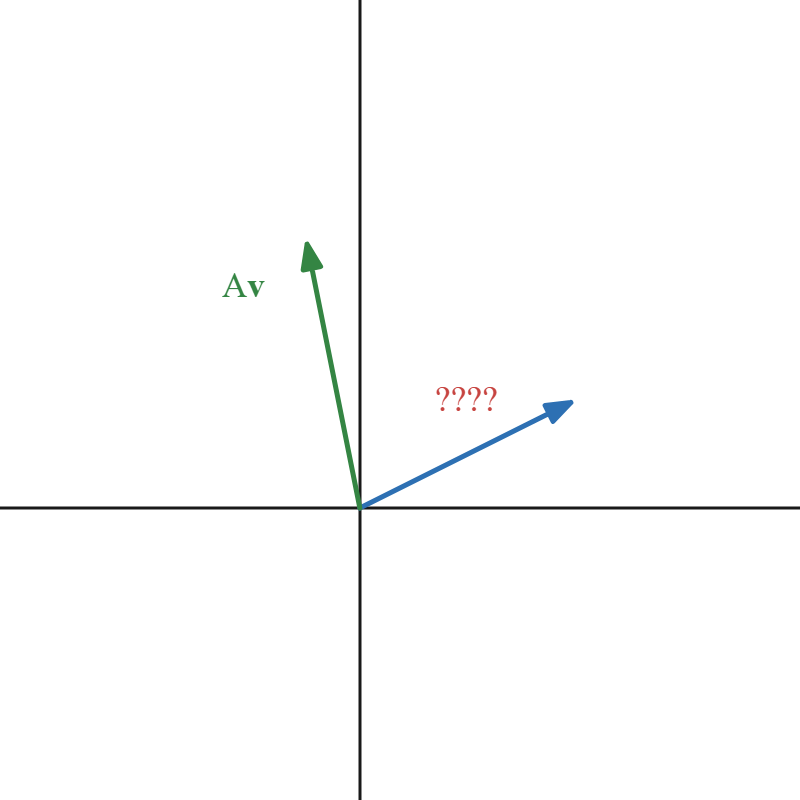
\includegraphics[width=0.5\linewidth]{chapters/chapter 3/inv.png}
\end{figure}

Այլ կերպ ասած՝ ունենալով $A$ մատրիցը, ինչո՞վ բազմապատկել $A\vv$ վեկտորը, որպեսզի ստացվի $\vv$։ Կամ՝
\[
\textbf{ի՞նչ} \; \times  \; A \; =\; I 
\]
Այդ \marginnote{$I$ ասելով նկատի ունենք համա\-պա\-տաս\-խան չափի միավոր մատրիցը} անհայտ ձևափոխությունը անվանում ենք $A$ գծային ձևափոխու\-թյան (կամ մատրիցի) \textit{հակադարձ} և նշանակում $A^{-1}$-ով։

\begin{definition}
Տրված $A$ մատրիցի \textbf{հակադարձ} կանվանենք այն $A^{-1}$ մատրիցը, որի համար
\[
AA^{-1} = A^{-1}A = I
\]
\end{definition}

Եթե գտնենք $A^{-1}$-ը, ապա կկիրառենք այն մեր ունեցած $A\vv$-ի վրա և կստանանք՝ $A^{-1}(A\vv) = (A^{-1}A)\vv=I\vv =\vv$:


\question{$A \in \R^{2 \times 2}$ գծային ձևափոխությունը վերցնում է վեկտորը և
\begin{enumerate}
    \item հորիզոնական ուղղությամբ ձգում $2$ անգամ,
    \item ապա $30^\circ$-ով պտտում,
    \item ապա ուղղաձիգ ուղղությամբ սեղմում $3$ անգամ,
    \item ապա ստացվածը շրջում $x$-երի առանցքի նկատմամբ։
\end{enumerate}
Հնարավո՞ր է ունենալով $\mathbf{v}=A\mathbf{u}$-ն՝ գտնել $\mathbf{u}$-ն։}

Պատասխանն է՝ այո, այսինքն՝ $A$ մատրիցն ունի հակադարձ (\textit{հակա\-դար\-ձելի} է)։ Ինչպես կտեսնենք, միայն որոշ քառակուսային մատրիցներ ունեն հակադարձ։

\question{Հակոբն իր հասակին գումարեց $6$, բազմապատկեց $0$-ով, հանեց $18$ և ստացավ $-18$ սմ։ Կարո՞ղ եք գտնել Հակոբի հասակը։}


\section{Որոշիչ}

Բնականաբար, հարց է առաջանում․ իսկ ինչպե՞ս գտնել տրված ձևա\-փոխու\-թյան հակադարձը, կամ առհասարակ ինչպե՞ս պարզել՝ այն ունի հակադարձ, թե ոչ։ 

Այդ նպատակով հետազոտենք մի այսպիսի տարօրինակ օբյեկտ։

\begin{definition}
\(2 \times 2\) չափանի
\[
  A = \begin{bmatrix}
    a & b \\
    c & d \\
  \end{bmatrix}
\]
մատրիցի \textbf{որոշիչ} կանվանենք\marginnote{անգլերեն՝ {\it determinant}} հետևյալ թիվը՝
\[
  \det(A) = ad - bc
\]
\end{definition}

\begin{example}
\[
  A = \begin{bmatrix}
    2 & 5 \\
    -3 & 4 \\
  \end{bmatrix}
\]
մատրիցի որոշիչն է՝ 
\[\det(A) = 2 \cdot 4 - 5 \cdot (-3) = 8+15=23\]
\end{example}

Փոքր-ինչ ավելի բարդ բանաձևով նաև $3 \times 3$ մատրիցի համար՝

\begin{definition}
\(3 \times 3\) չափանի
\begin{marginfigure}    \begin{center}

\includegraphics[width=\textwidth, height=\textheight, keepaspectratio]{chapters/chapter 3/det.png}
\end{center}
\end{marginfigure}\[
  A = \begin{bmatrix}
    a & b & c \\
    d & e & f \\
    g & h & i \\
  \end{bmatrix}
\]
մատրիցի որոշիչ կանվանենք հետևյալ թիվը՝
\[
  \det(A) = aei + bfg + cdh - ceg - bdi - afh
\]
\end{definition}

\begin{figure}[t]
\caption*{ձեռքով հաշվելիս հարմար է աջից արտագրել մատրիցի առաջին երկու սյուները, ապա հաշվել այսպես \bigskip }
\centering    {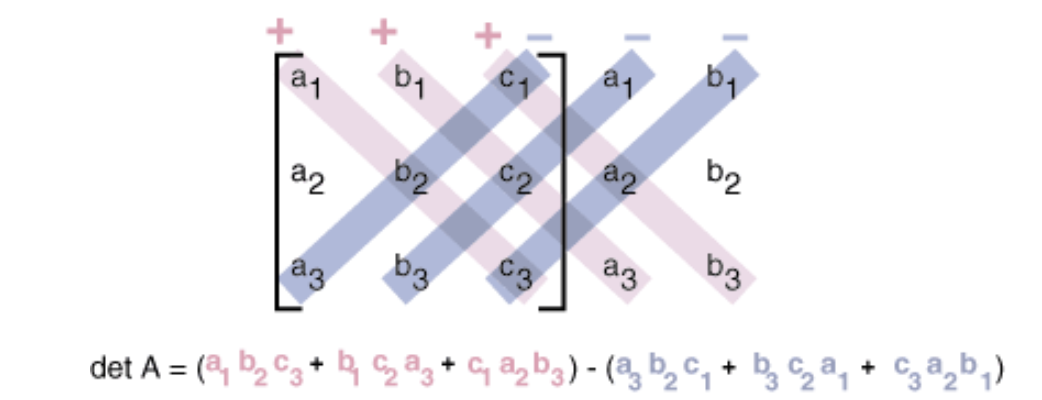
\includegraphics[width=0.8\linewidth]{chapters/chapter 3/det trick.png} }
\end{figure}

\begin{example}
\[
  A = \begin{bmatrix}
    1 & 2 & 3 \\
    4 & 5 & 6 \\
    7 & 8 & 9 \\
  \end{bmatrix}
\]
մատրիցի որոշիչն է՝ 
\[
  \det(A) = 1\cdot5 \cdot 9 + 2\cdot6\cdot7 + 3\cdot4\cdot8-3\cdot5\cdot7-2\cdot4\cdot9-1\cdot6\cdot8= 0
\]
\end{example}

Այսքանի վրա կանգ առնենք։ Ի՞նչ են ցույց տալիս այս բանաձևերը, ի՞նչ է նշանակում մատրիցի/ձևափոխության որոշիչը։

Դիտարկենք մեր $\R^2$ հարթությունը։ $x$-երի առանցքի վրա վերցնենք  \marginnote{միավոր $=$ $1$ երկարությամբ} $\ve_1=\begin{bmatrix}
    1 & 0
\end{bmatrix}$ միավոր վեկտորը, իսկ $y$-ների առանցքի վրա՝ $\ve_2=\begin{bmatrix}
    0 & 1
\end{bmatrix}$ միավոր վեկտորը։ Դրանցով կազմված փոքրիկ քառակուսին կանվանենք \textit{միավոր քառակուսի։}

\begin{figure}[h]
    \centering
    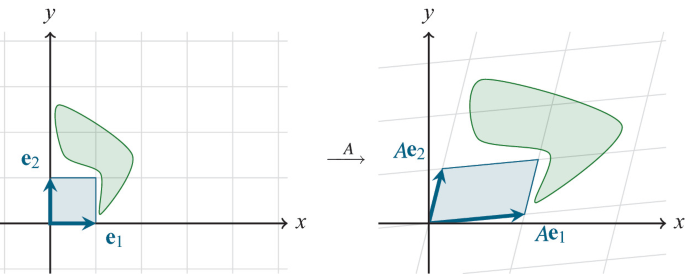
\includegraphics[width=0.75\linewidth]{chapters/chapter 3/viz area.png}
\end{figure}

$A$ ձևափոխությունը կիրառելուց հետո $\ve_1$-ն ու $\ve_2$-ը պտտվելով-ձգվելով վերածվում են $A\ve_1$ և $A\ve_2$ վեկտորների։ Քանի որ միավոր քառակուսին կազմված էր այդ երկու վեկտորներով, ապա այն նույնպես ձևափոխվում է (պտտվում-ձգվում և այլն) ու դառնում արդեն $A\e_1$ և $A\e_2$ վեկտորներով ստացվող \textit{զուգահեռագիծ։}

Եթե ձևափոխությունից առաջ միավոր քառակուսու մակերեսը $1$ էր, ապա ձևափոխությունից հետո ստացված զուգահեռագծի մակերեսը $|\det(A)|$ է։ Ավելին, ոչ միայն միավոր քառակուսու, այլ \textit{ցանկացած} պատկերի դեպքում՝ երբ կիրառում ենք $A$ ձևափոխությունը\marginnote{մտքում պատկերացրեք կետերի շարժը}, այն փոփոխվում է, իսկ նրա մակերեսը մեծանում/փոքրանում է $|\det(A)|$ անգամ։

Այսինքն՝ յուրաքանչյուր գծային ձևափոխություն կիրառելիս պատկերների մակերեսները որոշ չափով ձգվում կամ սեղմվում են, և նրա որոշիչը ցույց է տալիս, \marginnote{փաստորեն օրինակ՝ \hyperref[mona]{\color{OliveGreen} $M$ ձևափոխության արդյունքում} Մոնա Լիզան մեծանում է $\det(M)=1.89$ անգամ}\textit{թե քանի անգամ են մակերեսները ձգվում․} որոշիչը հենց այդ ձգման գործակիցն է (անգլերեն՝ {\it scaling factor})։ 

\question{Որքա՞ն է $I_n$ նույնական ձևափոխության որոշիչը։}

Արդեն իմանալով որոշիչի իմաստը՝ ձևակերպենք դրա հատկությունները։

\begin{theorem}
Ցանկացած $n \times n$ չափանի  $A$, $B$ մատրիցների համար

\begin{enumerate}
\item $\det(cA) = c^n \cdot \det(A)$ ցանկացած $c\in\R$ թվի համար\marginnote{$n$-ը մատրիցի չափն է} 

\item $\det(AB) = \det(A) \cdot \det(B)$ 

\item եթե $A$-ն ունի հակադարձ, ապա $\det(A^{-1}) = \dfrac{1}{\det(A)}$

\item $\det(I)=1$

\item $\det(A^T) = \det(A)$

\item եթե $A$-ի տողերից/սյուներից որևէ մեկը բաղկացած է միայն $0$-ներից, ապա $\det(A)=0$

\item եթե $\det (A) <0$, ապա $A$-ն նաև շրջում է տարածությունը։
\end{enumerate}
\end{theorem}

\question{Ինչո՞ւ են ճիշտ 1-4 հատկությունները։}

Նշենք, որ $4 \times 4$, $5 \times 5$ և ավելի մեծ չափանի քառակուսային մատրիցների որոշիչները հաշվելու համար նույնպես կան տարբեր բանաձևեր (իսկ ոչ քառակուսային մատրիցները \textbf{որոշիչ չունեն}), բայց դրանց հաշվողական մասը մեզ հետաքրքիր չէ։ Օգտակար կլինի նաև իմանալ, որ
\begin{theorem}
Եթե մատրիցի տողերից կամ սյուներից որևէ մեկը
\begin{itemize}
\item բազմապատկենք ինչ-որ $c$ թվով, ապա որոշիչը կմեծանա $c$ անգամ,

\item գումարենք որևէ այլ տողի/սյան, ապա որոշիչը չի փոխվի։
\end{itemize}
\end{theorem}

\section{Հակադարձելիություն}

Իսկ ի՞նչ, եթե գծային ձևափոխության որոշիչը $0$ է։

\begin{figure}[h]
    \centering
    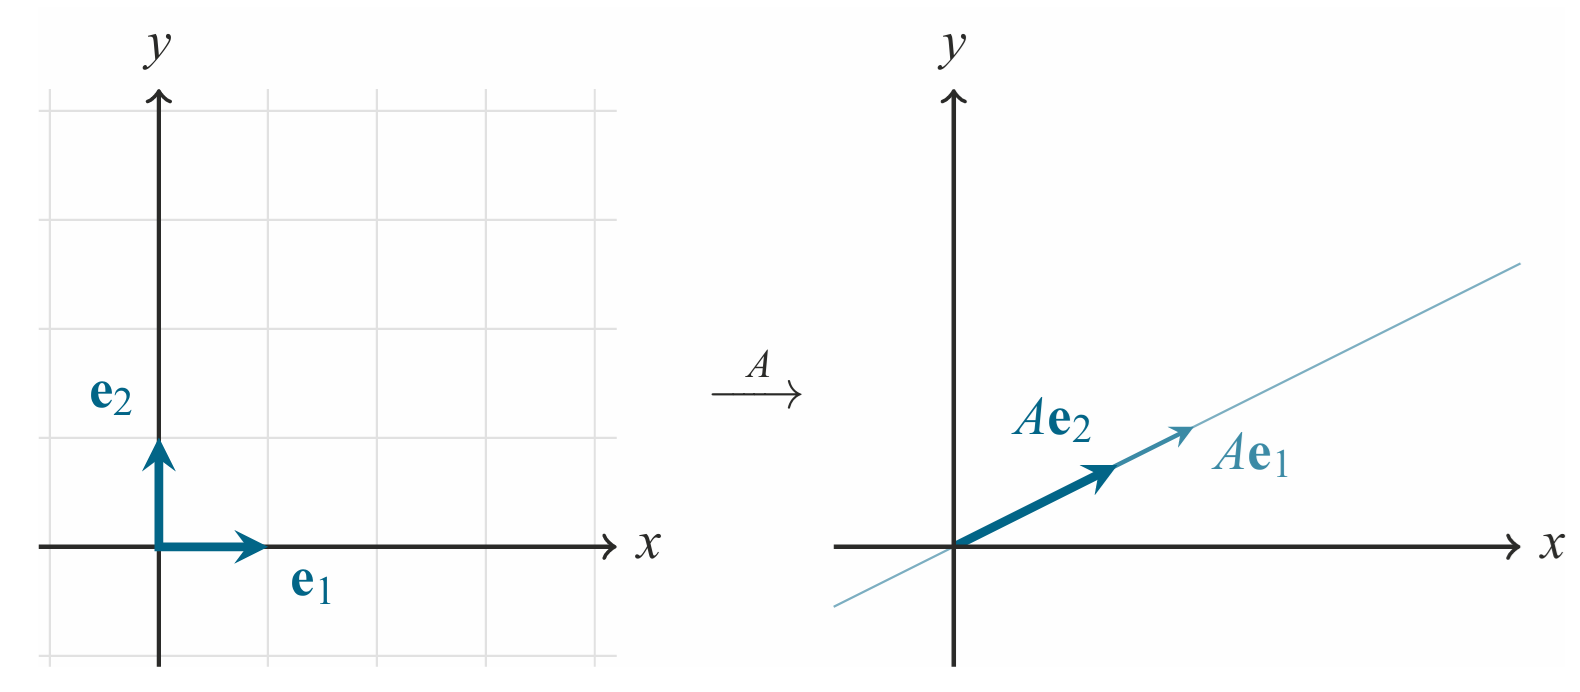
\includegraphics[width=0.75\linewidth]{chapters/chapter 3/0 det.png}
\end{figure}

Նշանակում է՝ ցանկացած պատկերի մակերեսը ձևափոխությունից հետո դառնում է $0$։ Այսինքն ձևափոխությունը տարածության մեջ եղած ամեն ինչ սեղմում-ճզմում է՝ դարձնելով զրո մակերեսով ինչ-որ բան\marginnote{$\R^3$-ի դեպքում՝ նաև հարթություն} ($\R^2$-ի դեպքում՝ ուղիղ կամ պարզապես կետ)։

\question{$A$ մատրիցը յուրաքանչյուր $[x \quad y]$ վեկտորի տանում է դեպի $[x \quad 0]$։ Ո՞ր վեկտորները $A$-ն կիրառելիս կդառնան $[7 \quad 0]$:}  
Այս դեպքում եթե վերցնենք որևէ $\vv$ վեկտոր, կիրառենք $A$-ն (ճզմելով տարածությունը) և փորձենք $A\vv$-ից հետ գնալ դեպի սկզբնական $\vv$ վեկտորը, ապա որքան էլ ուզենք՝ չենք կարող պարզել, թե որն էր $\vv$-ն, քանի որ $\vv$-ի հետ նույն գծի վրա գտնվող բազմաթիվ այլ վեկտորներ ևս ճզմվելով դարձել են $A\vv$։

\begin{theorem}
$A$ քառակուսային\marginnote{ոչ քառակուսային մատրիցները ևս հակադարձ չունեն} մատրիցն ունի հակադարձ այն և միայն այն դեպքում, եթե $\det(A) \ne 0$:
\end{theorem}

Ինչպես կարող ենք ստուգել, $2 \times 2$ չափանի 
\[
\begin{bmatrix}
    a & b \\ c & d
\end{bmatrix}
\]
մատրիցի հակադարձը (եթե $\det(A)\ne 0$) կարելի է գտնել հետևյալ բանաձևով՝\marginnote{ստուգեք, որ $AA^{-1}=I_2$}
\[
A^{-1} = \frac{1}{\det(A)} \begin{bmatrix} d & -b \\ -c & a \end{bmatrix}
\]

\begin{example}
$A = \begin{bmatrix} 2 & 3 \\ 1 & 4 \end{bmatrix}$ մատրիցը հակադարձելի է և
\[
A^{-1} = \frac{1}{\det A} \begin{bmatrix} 4 & -3 \\ -1 & 2 \end{bmatrix} = \frac{1}{5} \begin{bmatrix} 4 & -3 \\ -1 & 2 \end{bmatrix}=\begin{bmatrix}
    0.8 & -0.6 \\ -0.2 & 0.4
\end{bmatrix}
\]
\end{example}

\question{Սկզբից կիրառել ենք $A$ ձևափոխությունը, այնուհետև $B$-ն, և ստացել ենք $\vu$։ Ինչպե՞ս գտնենք սկզբնական վեկտորը։}

Ավելի մեծ չափանի հակադարձները հաշվելու համար նույնպես կան բավական հետաքրքիր բանաձևեր և ալգորիթմներ, բայց մենք դրանց նույնպես ուշադրություն չենք դարձնի։ Նկատենք միայն, որ
\[
\left(AB\right)^{-1} = B^{-1}A^{-1}
\]

\section{Հետք}

Որոշիչից բացի սահմանենք նաև մատրիցի հետքը։

\begin{definition}
$A$ քառակուսային մատրիցի \textbf{հետք} կանվանենք նրա անկյունագծի վրա գրված տարրերի գումարը՝\marginnote{անգլերեն՝ {\it trace}}
\[
\operatorname{tr}(A) = a_{11} + a_{22} + \ldots + a_{nn}
\]
\end{definition}

\begin{example}
\[
  A = \begin{bmatrix}
    2 & 5 & 1 \\
    0 & -3 & 4 \\
    7 & 2 & 6 \\
  \end{bmatrix}
\]
մատրիցի հետքն է՝
\[
  \operatorname{tr}(A) = 2 + (-3) + 6 = 5
\]
\end{example}

Ի՞նչ է ցույց տալիս հետքը։ Այս մասին կխոսենք ավելի ուշ։ Առայժմ ֆիքսենք դրա հատկությունները։

\begin{theorem}
Ցանկացած $n \times n$ չափանի  $A$, $B$ մատրիցների համար

\begin{enumerate}
\item \(\operatorname{tr}(cA) = c \cdot \operatorname{tr}(A)\) ցանկացած $c\in \R$ թվի համար

\item \(\operatorname{tr}(A + B) = \operatorname{tr}(A) + \operatorname{tr}(B)\)

\item \(\operatorname{tr}(AB) = \operatorname{tr}(BA)\) 

\item \(\operatorname{tr}(A^T) = \operatorname{tr}(A)\)
\end{enumerate}
\end{theorem}

Ինչպես տեսնում ենք, մատրիցի հետքը հարուստ է շատ օգտակար հատկություններով։ Ինչ-որ իմաստով՝ նրա սահմանումը միակն է, որ կարող է բավարարել բոլոր վերոնշյալ $4$ հատկություններին։



\bigskip 

\begin{theory}
.
\begin{itemize}
\item կարդալ [{\rm Poole}], 221-223 էջերը (ձևափոխության հակադարձ)
\item կարդալ [{\rm Johnston}], 254-256 (հետք), 258-263 (որոշիչ) էջերը  
\item դիտել  {\rm 3b1b}-ի \href{https://www.3blue1brown.com/lessons/matrix-multiplication}{4-րդ} և \href{https://www.3blue1brown.com/lessons/determinant}{6-րդ} տեսադասերը գծային հանրահաշվից 
\item ըստ ցանկության՝ նաև \href{https://www.3blue1brown.com/lessons/inverse-matrices}{7-րդը}
\item տեսնել որոշ մատրիցներ \href{https://intuitive-math.club/linear-algebra/matrices}{սեփական աչքով}
\end{itemize}
\end{theory}

\newpage

\section{Խնդիրներ}

\begin{problem}
Ձևափոխության նկարագրությունը համապատասխանեցրեք իր մատրիցին․ 

\textit{Նկարագրություն՝} 

\begin{enumerate}[label={\alph*}․]
\item պտտում է $70^\circ$-ով
\item ոչինչ չի անում
\item շրջում է $x$-երի առանցքի շուրջ
\item $y$-ների ուղղությամբ ձգում է $5$ անգամ
\item ամեն բան տանում է $y=6x$ ուղղի վրա
\item ամեն բան տանում է $y=6x+1$ ուղղի վրա
\end{enumerate}

\setlength{\columnseprule}{0pt}

\textit{Մատրից՝} 
\begin{multicols}{2}
\begin{enumerate}
\item $\begin{bmatrix}
    1&0\\0&5
\end{bmatrix}$\vfill
\item այդպիսի մատրից չկա\vfill
\item $\begin{bmatrix}
    1&0\\0&1
\end{bmatrix}$
\item $\begin{bmatrix}
    0.342 & -0.939\\
     0.939& 0.342
\end{bmatrix}$
\item $\begin{bmatrix}
    1&0\\0&-1
\end{bmatrix}$
\item $\begin{bmatrix}
    3&-1\\18&-6
\end{bmatrix}$
\end{enumerate}
\end{multicols}


\hint{Հաշվեք որոշիչները։ Հետևեք նաև, թե ո՞ւր է գնում $\mathbf{0}$-ն։}
\end{problem}

\begin{problem}
Ինչի՞ է հավասար մատրիցի որոշիչը, եթե այն
    
\begin{enumerate}[label={\alph*}․]
\item ամեն ինչ պտտում է $14^\circ$-ով և $1.5$ անգամ ձգում $x$-երի ուղղությամբ

\item \textit{ա․} մատրիցի հակադարձն է

\item $\begin{bmatrix}
    1 & 0
\end{bmatrix}$ վեկտորը տանում է $\begin{bmatrix}
    2 & 4
\end{bmatrix}$, իսկ $\begin{bmatrix}
    0 & 1
\end{bmatrix}$-ը՝ $\begin{bmatrix}
    -1 & 0
\end{bmatrix}$

\item ունի հետևյալ տեսքը՝ $\begin{bmatrix}
2 & 3 \\ 2 &1
\end{bmatrix}$

\item ունի հետևյալ տեսքը՝ $\begin{bmatrix}
8&3&5\\1&4&2\\-4&0&4   \end{bmatrix}$

\item \textit{ե․} մատրիցն է՝ բարձրացրած խորանարդ
\end{enumerate}
\end{problem}


\begin{problem}
Եթե վերցնենք $x^2+y^2=1$ միավոր շրջանագիծը և $2$ անգամ ձգենք $x$-երի առանցքի ուղղությամբ,\marginnote{$(0,0)$ կենտրոնով և $1$ շառավղով} արդյունքում կստանանք \textit{էլիպս։} Որքա՞ն կլինի դրա մակերեսը։

\begin{figure}[!h]
    \centering
    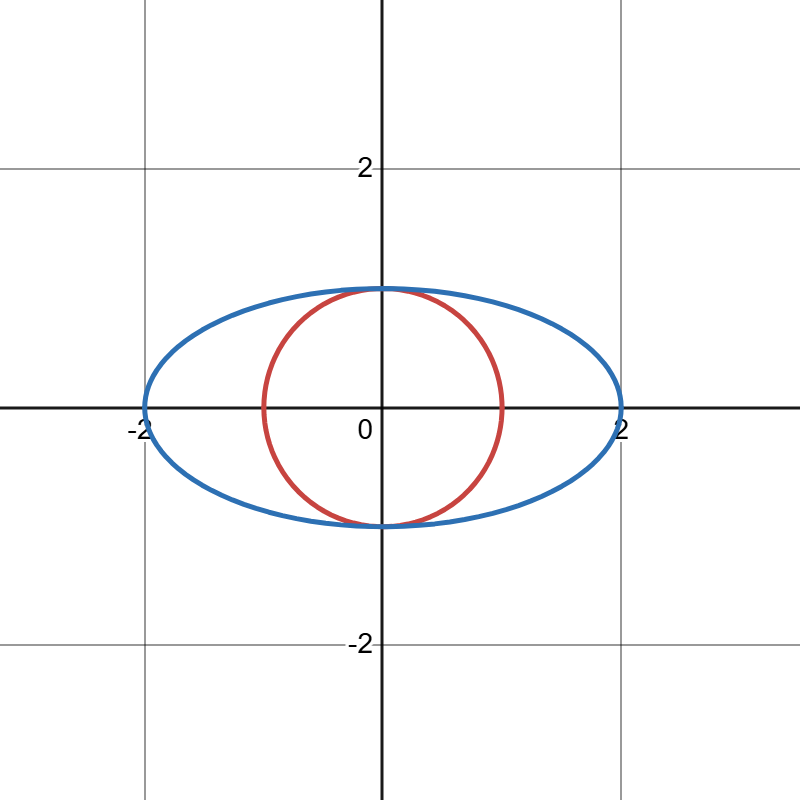
\includegraphics[width=0.45\linewidth]{chapters/chapter 3/ellipse.png}
\end{figure}

Կարո՞ղ եք ընդհանրացնելով արդյունքը՝ ստանալ բանաձև էլիպսի մակերեսի համար։
\end{problem}


\begin{problem}
Հայտնի է, որ
\[
A=\begin{bmatrix}
    4 & -8 \\ 1 & 2
\end{bmatrix}
\]
մատրիցը ինչ-որ $\mathbf{v}$ վեկտորի տանում է դեպի
\begin{enumerate}[label={\alph*}․]
\item $\begin{bmatrix}
    1 \\2
\end{bmatrix}$
\item $\begin{bmatrix}
    3 \\ 4
\end{bmatrix}$
\end{enumerate}
Կարո՞ղ եք գտնել $\mathbf{v}$ վեկտորը։
\end{problem}

\begin{problem}
Ենթադրենք տրված է 
\[
A=\begin{bmatrix}
    a & b \\ c & d
\end{bmatrix}
\]
\begin{marginfigure}
    \caption*{այս գծագիրը կարող է օգնել}
    \centering
    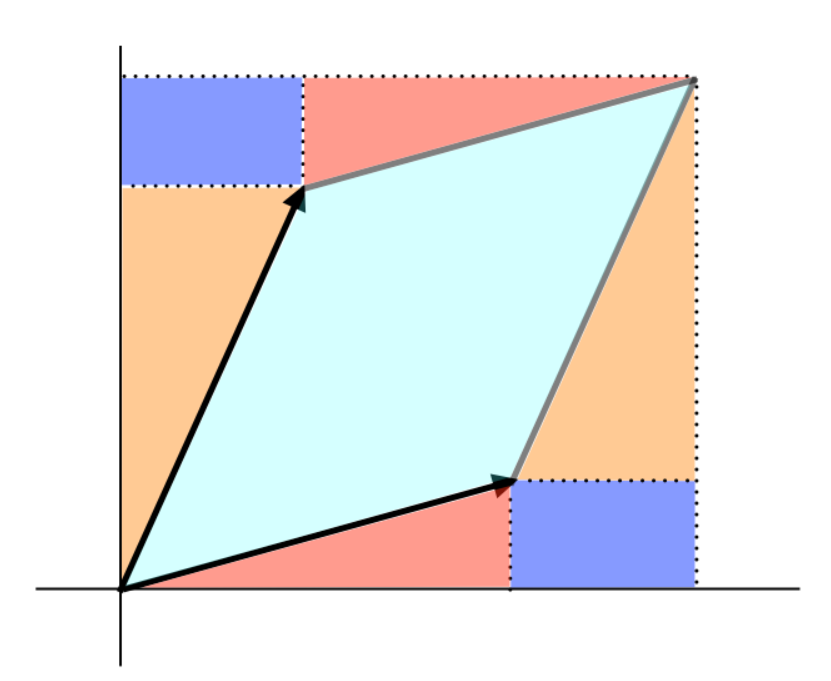
\includegraphics[width=\linewidth]{chapters/chapter 3/det explained.png}
\end{marginfigure}
մատրիցը։ $A$-ն կիրառելիս 
\begin{enumerate}[label={\alph*}․]
\item որտե՞ղ է գնում $\begin{bmatrix}
    1 & 0
\end{bmatrix}$ վեկտորը

\item որտե՞ղ է գնում $\begin{bmatrix}
    0 & 1
\end{bmatrix}$ վեկտորը

\item ինչո՞ւ է դրանցով ստացված զուգահեռագծի մակերեսը հավասար $|\det(A)|$-ին
\end{enumerate}
\end{problem}


\begin{problem}
Ինչպես գիտենք, ցանկացած մատրից միավոր մատրիցով բազմապատկելիս մնում է նույնը։ Տեղերով փոխենք $I_4$ մատրիցի երկրորդ և երրորդ տողերը՝
\[
B = \begin{bmatrix}
    1 & 0 & 0 & 0 \\
    0 & 0 & 1 & 0 \\
    0 & 1 & 0 & 0 \\
    0 & 0 & 0 & 1
\end{bmatrix}
\]
\begin{enumerate}[label={\alph*}․]
\item ի՞նչ է լինում $4 \times 4$ չափի մատրիցի հետ, երբ այն բազմապատկում ենք $B$-ով (ենթադրենք՝ ձախից)

\item որքա՞ն է $B$-ի որոշիչը

\item ինչպե՞ս է փոխվում մատրիցի որոշիչը, երբ նրա երկրորդ ու երրորդ տողերը տեղերով փոխում ենք

\item ինչպե՞ս կընդհանրացնեք ստացված արդյունքը
\end{enumerate}
\end{problem}
